\chapter{КОНСТРУКТОРСКАЯ ЧАСТЬ}

\section{Диаграмма IDEF0}

На рисунке~\ref{fig:idef0} изображена диаграмма IDEF0 для требуемой задачи:

\begin{figure}[H]
	\centering
	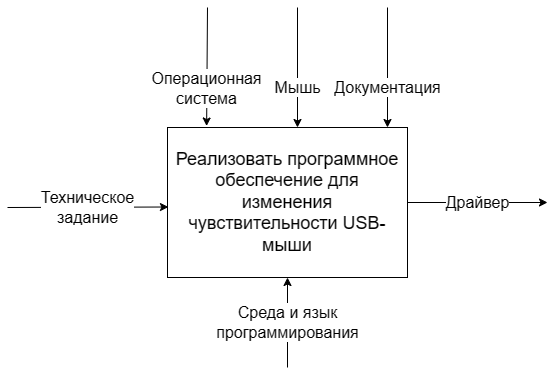
\includegraphics[width=0.9\linewidth]{inc/idef0.png}
	\caption{Диаграмма IDEF0}
	\label{fig:idef0}
\end{figure}

\section{Алгоритм перехвата событий мыши}

На рисунке~\ref{fig:algo} изображена схема алгоритма перехвата событий мыши.
\captionsetup{justification=centering,singlelinecheck=false}
\begin{figure}[H]
	\centering
	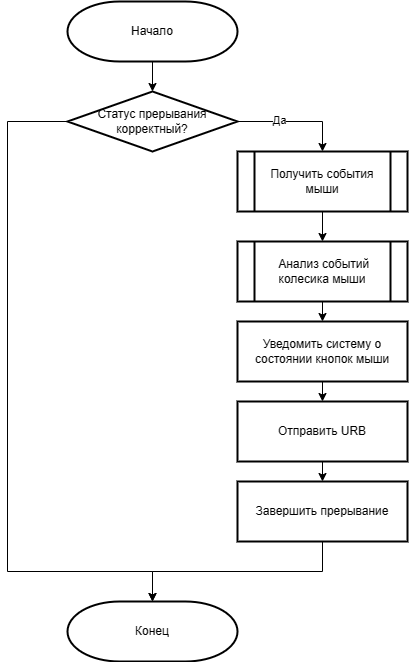
\includegraphics[width=0.7\linewidth]{inc/algo}
	\caption[]{Схема алгоритма перехвата событий мыши}
	\label{fig:algo}
\end{figure}

\section{Алгоритм анализа событий колесика мыши}

На рисунке~\ref{fig:algo-wheel} изображена схема алгоритма анализа событий колесика мыши.
\captionsetup{justification=centering,singlelinecheck=false}
\begin{figure}[H]
	\centering
	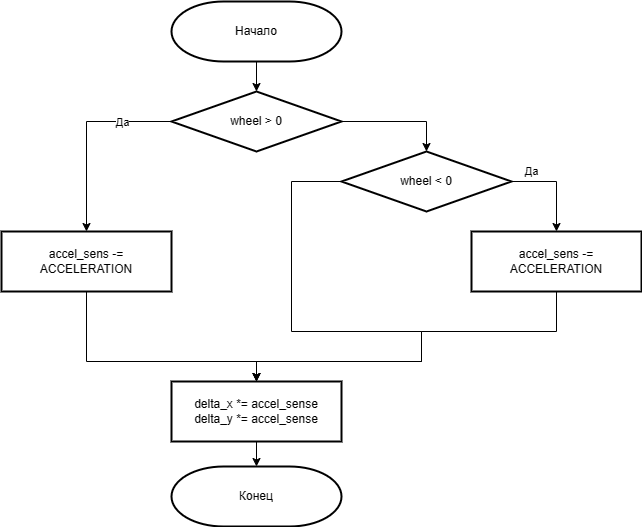
\includegraphics[width=0.8\linewidth]{inc/algo-wheel}
	\caption[]{Схема алгоритма анализа событий колесика мыши}
	\label{fig:algo-wheel}
\end{figure}